\documentclass[10pt,letterpaper]{article}
% Add a bunch of useful math, font, and symbols
\usepackage{amsfonts}
\usepackage{amsmath}
\usepackage{amssymb}

% English support
\usepackage[english]{babel}

% Citation
\usepackage[superscript]{cite}

% Better enumerate and itemize
\usepackage{enumitem}

% Better control of headers and footers
\usepackage{fancyhdr}

% Floating objects like figures and tables
\usepackage{float}

% Page layout and dimensioning
\usepackage[margin=1in]{geometry}

% Basic color, graphics and text manipulation 
\usepackage{graphicx}

% Use Helvetica typeface
\usepackage[scaled]{helvet}
\renewcommand\familydefault{\sfdefault} 
\usepackage[T1]{fontenc}

% Cross-referencing hyperlinks
\usepackage{hyperref}

% Line break for long URLs
\usepackage{breakurl}

% Accept utf-8 input encoding
\usepackage[utf8]{inputenc}

% Make indexes
\usepackage{makeidx}

% Microtype (apparently makes the typographics stuff better)
\usepackage{microtype}

% [Disabled] multi-column writing
% \usepackage{multicol}

% English ordinal counting (1st, 2nd, etc.)
\usepackage{nth}

% Long table
\usepackage{longtable}

% Paragraph skip - adds extra lineskip spacing
\usepackage{parskip}
\setlength{\parskip}{0.7\baselineskip plus 2pt}

% Add ability to set space between lines
\usepackage{setspace}

% S.I. units
\usepackage{siunitx}

% Subcaptions for subfigures
\usepackage{subcaption}

% Include svg graphics
\usepackage{svg}

% Drawing graphics
\usepackage{tikz}

% Subsubsubsection
\usepackage{titlesec}
\setcounter{secnumdepth}{4}
\titleformat{\paragraph}
{\normalfont\normalsize\bfseries}{\theparagraph}{1em}{}
\titlespacing*{\paragraph}
{0pt}{3.25ex plus 1ex minus .2ex}{1.5ex plus .2ex}

% Custom titles
\usepackage{titling}

% Url
\usepackage{url}

\RequirePackage[figure,table]{totalcount}


% Custom definitions
\newcommand{\doctitle}{Operations, Maintenance, and Upgrades Specification}
\newcommand{\docsubtitle}{Computing Platform Multirotor with FPGA Hardware Acceleration Applications}
% Custom commands
\newcommand{\ts}{\textsubscript}	% Subscript command %


% Use hyphans to break up urls
\def\UrlBreaks{\do\/\do-}

% PDF and href setup
% Hyper ref
\hypersetup{
	colorlinks=true,
	citecolor=black,
	linkcolor=black,
	filecolor=black,
	urlcolor=blue,
	pdftitle={\@title},
	bookmarks=true
}
\urlstyle{same}
% Page headings
\pagestyle{fancy}
\fancyhead[L]{\MakeUppercase{CPEN/ELEC 491}}
\fancyhead[C]{\textbf{\doctitle}}
\fancyhead[R]{Mieszko Lis, PhD}
\fancyfoot{}
\fancyfoot[C]{Non-Confidential}
\fancyfoot[R]{\thepage}

% No paragraph indent
\parindent 0ex

% Meta
\author{
	Deutsch, Peter &
	\textit{me@peterdeutsch.ca}
	\\
	He, Muchen &
	\textit{m.he@alumni.ubc.ca}
	\\
	Hsueh, Arthur &
	\textit{ah11962@outlook.com}
	\\
	Wang, Meng &
	\textit{wzfftxwd@gmail.com}
	\\
	Wilson, Ardell &
	\textit{ardellw96@gmail.com}
}
\title{\doctitle}
\date{\today}
\makeatletter
\renewcommand{\maketitle}{
	\bgroup
	\setlength{\parindent}{0pt}
	\begin{flushleft}
		% Top spacing
		\vspace*{0.5in}

		% Team logo
		
\includegraphics[scale=0.4]{../assets/capstonelogo1.png}
		\vspace*{0.25in}

		% Title
		\textbf{\Huge{\@title}}\\
		\hrulefill

		% Subtitle
		\textbf{\huge{\docsubtitle}}
		
		\vspace*{0.5in}

		% Course number and team
		\textbf{\Large{CPEN/ELEC 491 Capstone Team 109}}\\
		\hspace*{0.1cm}
		\begin{tabular}[h]{|ll}
			\@author
		\end{tabular}

		\vspace*{0.25in}

		\textbf{\Large{Mieszko Lis, PhD}}\\
		\hspace*{0.1cm}
		\begin{tabular}[h]{|ll}
			Electrical and Computer Engineering, The University of British Columbia
		\end{tabular}

		\vfill
		
		% Date
		\large{Revision 1.0 -- \@date}
		\vspace*{0.5in}

		% Logo
		\hspace*{-0.3cm}
\includegraphics[scale=0.5]{../assets/ece_logo.pdf}

	\end{flushleft}
	\egroup
}
\makeatother

% Begin Document
\begin{document}

% Title Page
\begin{titlepage}
	\maketitle
\end{titlepage}


\renewcommand{\thepage}{\roman{page}}
\setcounter{page}{1}

% Revision history
\backgroundsetup{
	scale=1,
	color=black,
	opacity=0.3,
	angle=0,
	contents={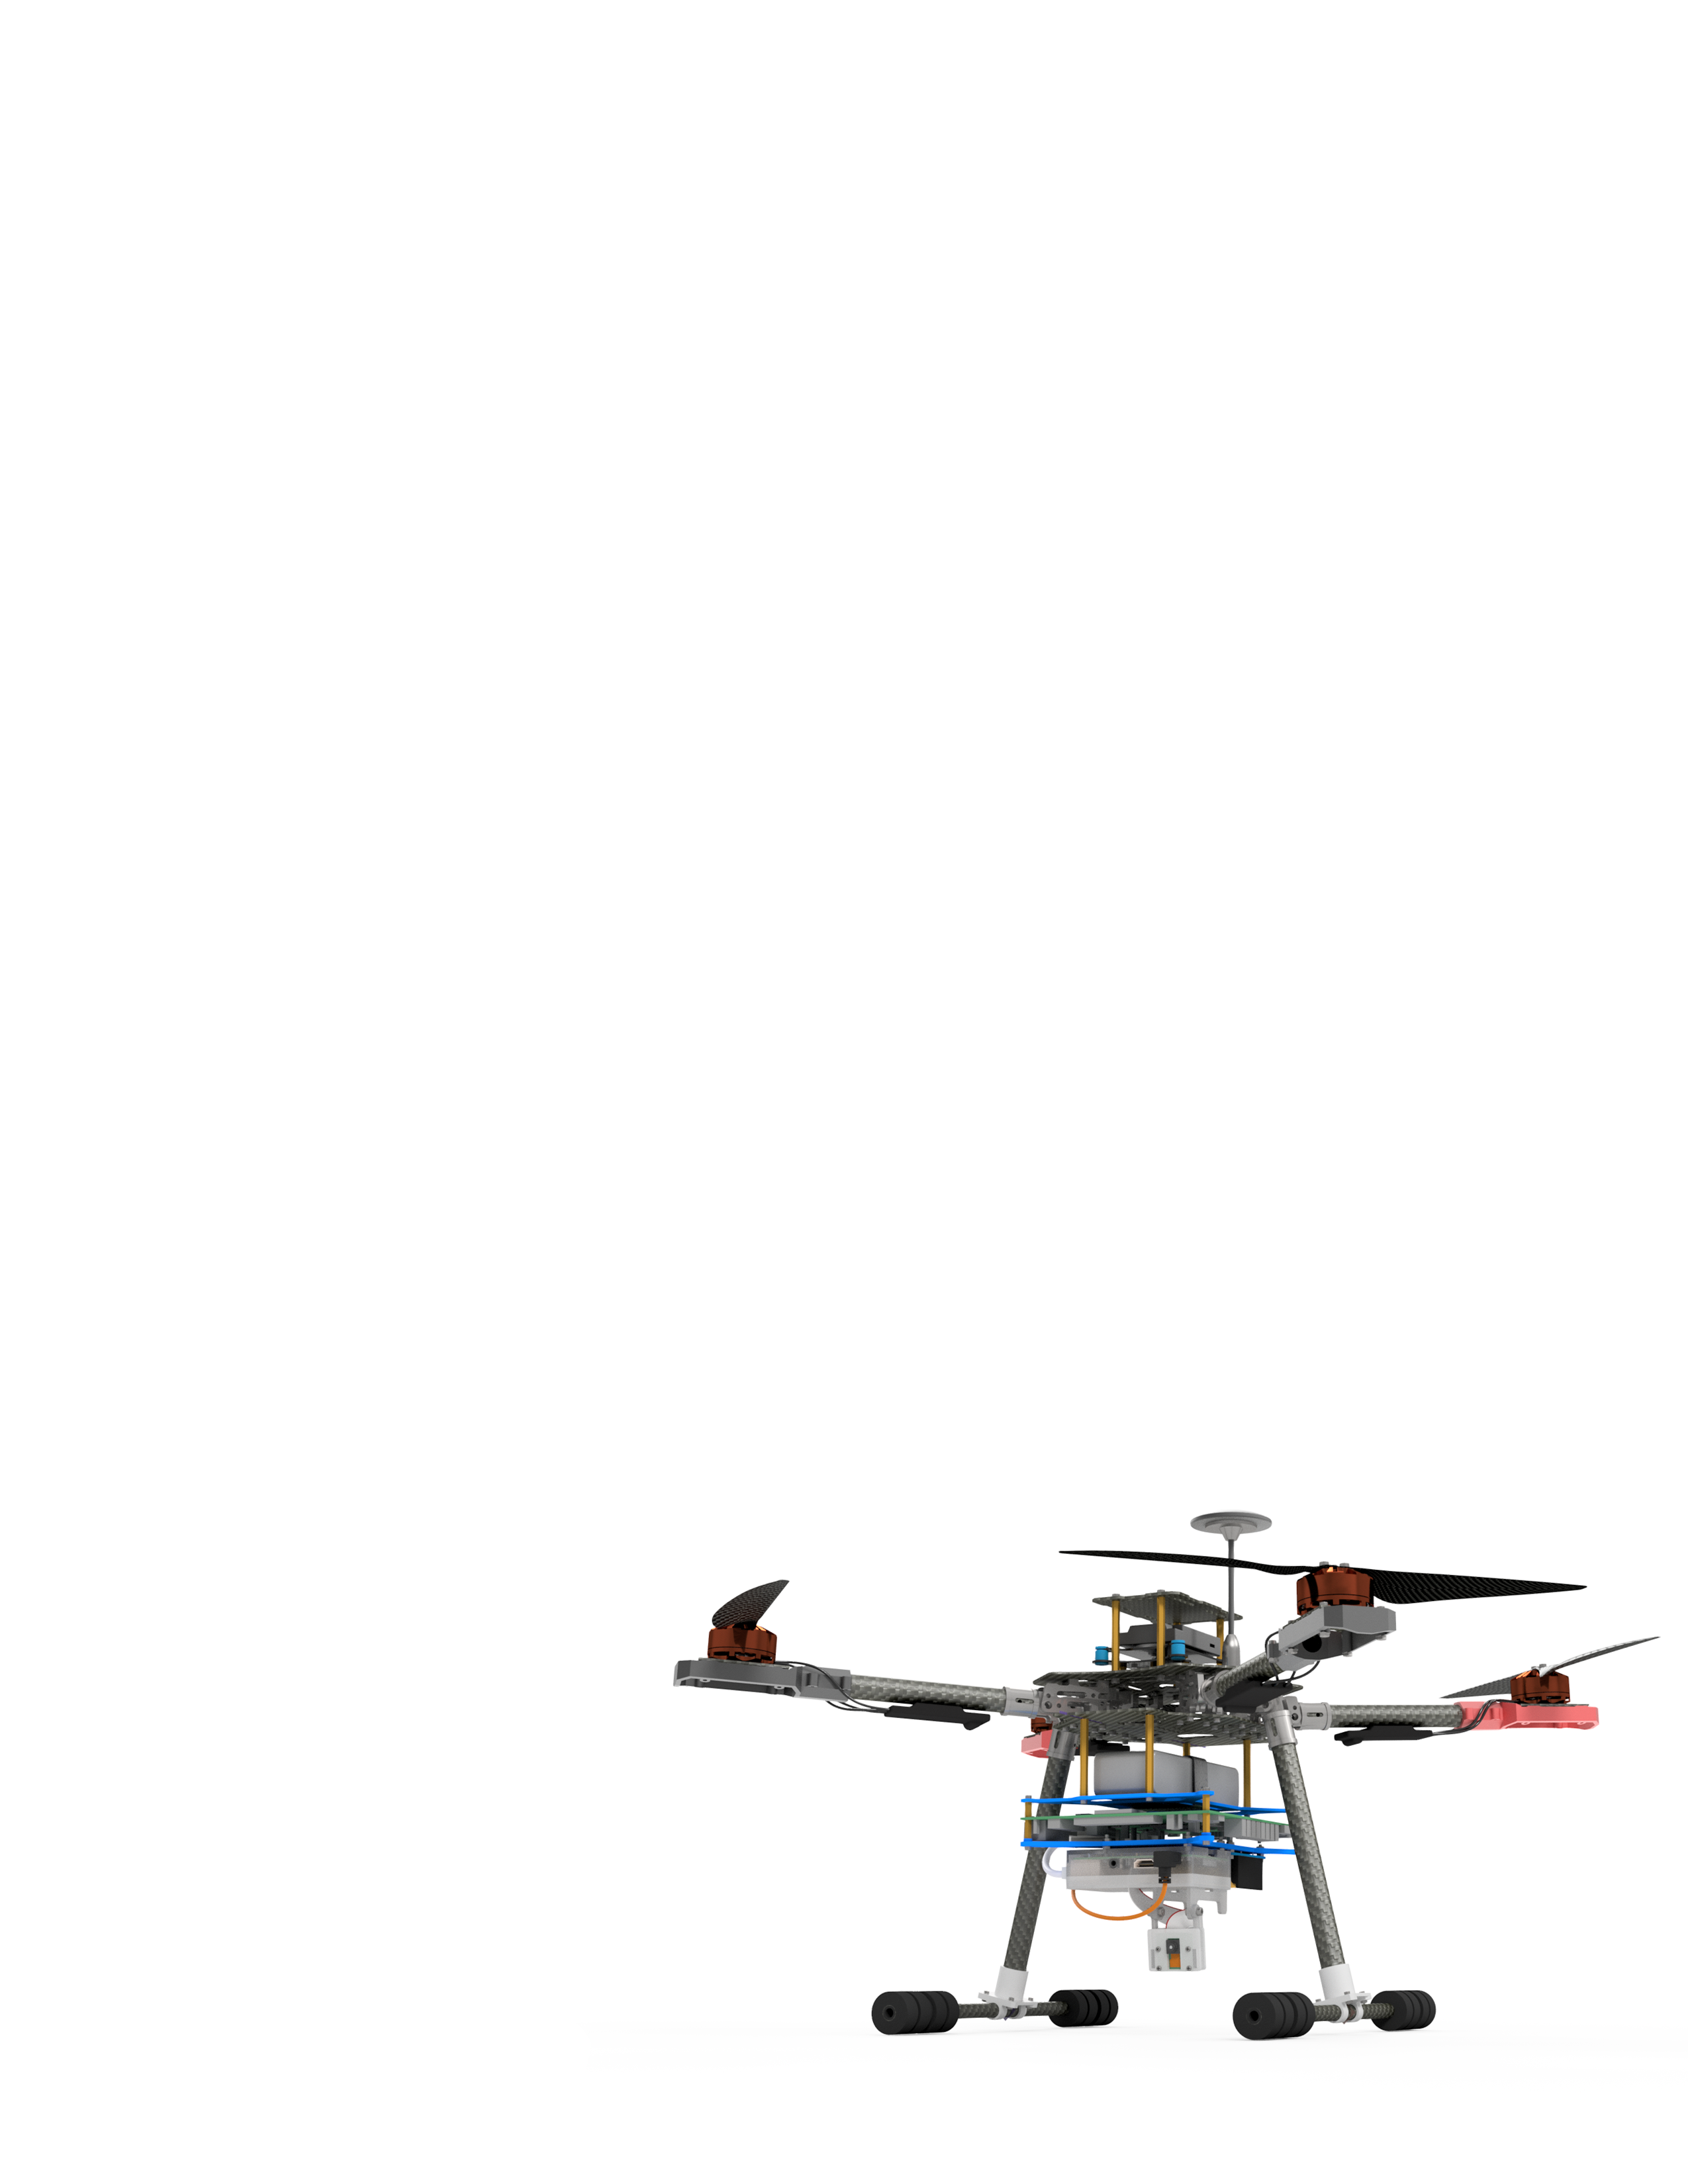
\includegraphics[height=\paperheight,width=\paperwidth]{../assets/render2bg}}
}
\BgThispage
%\thispagestyle{empty}
\section*{Revision History}
The full revision history and commited changes of the document can be found in the git repository history: \href{https://github.com/Capstone-Skynet/Capstone-Skynet.github.io}{https://github.com/Capstone-Skynet/Capstone-Skynet.github.io/commits/master}.

\begin{table}[H]
\begin{tabular}{*{4}{l}p{0.5\linewidth}}
\hline
Version \# & Initials & Release Date & Changeset & Changes Made \\ \hline

0.0 & PD & 2019-10-11 & \texttt{660e001} & Initial skeleton of the document.\\
0.1 & MH & 2019-10-11 & \texttt{6af9e8a} & Populate initial document with draft content required for Milestone I.\\
0.2 & PD & 2019-11-23 & & Initial framework for test descriptions created.\\
0.3 & MW & 2019-11-24 & & First set of tests added.\\
1.0 & PD & 2019-11-25 & & General clean-up and release for Milestone II.\\
1.1 & AH & 2020-02-09 & & Added Full System Tests \\

 & & & \\ \hline
\end{tabular}
\end{table}
\clearpage

% Table of contents
\setcounter{secnumdepth}{3}
\tableofcontents

% Roman numeral page numbers


% Terms and Abbreviations
\thispagestyle{empty}

\section*{Terms and Abbreviations}

Technical terms and abbreviations dictionary go here.

\begin{tabular}[h]{rp{0.75\linewidth}}
    \hline
    \textbf{Term} & \textbf{Definition}\\
    \hline

    ANN & Artificial Neural Network, or simply ``Neural Network'', is a data processing model modeled after neuron interactions. The process consists of forward propagation using several matrix multiplications.\cite{ann}\\
    ASIC & Application-specific Integrated Circuits.\\
    CNN & Convolutional neural network are neural networks that is especially useful for image classification.\cite{cnn} \\
    ECE & Department of Electrical and Computer Engineering at the University of British Columbia.\\
    FPGA & Field-Programmable-Gate-Arrays, ``programmable'' hardware that allows ASIC-like performance with software-like turn-around time and flexibility.\\
    GPU & Graphics Processing Unit, a discrete piece of hardware designed to accelerate graphic-intensive or other parallel computing tasks.\\
    LOS & Line-of-sight.\\
    ML & Machine learning.\\
    Multirotor & An unmanned vehicle with multiple engines. \\
    OTS & Off-the-shelf, or commercially available/purchasable \\
    PID / PID Controller & Proportion-Integral-Derivative controllers is the most common control algorithm for precise and accurate movement, as well as to compensate external forces.\cite{pid}\\
    RNN & Recurrent neural networks are neural networks where the output depends on previous computations, essentially consists of memory.\cite{rnn}\\
    RX & Receiver.\\
    TC & Transport Canada.\\
    TX & Transmitter.\\
    YOLO & You-Only-Look-Once is a fast ML algorithm that detect objects but is unlike CNN nor RNN.\cite{yolo}\cite{yolo-2}\\
     & \\

    \hline

\end{tabular}


% List of figures and tables
\iftotalfigures
\addcontentsline{toc}{section}{\listfigurename}
\listoffigures
\fi
\iftotaltables
\addcontentsline{toc}{section}{\listtablename}
\listoftables
\fi

\newpage

% Set page and section counter
\renewcommand{\thepage}{\arabic{page}}
\setcounter{page}{1}

% TODO: fill out all the sections
% if the sections gets too long, move them to a separte .tex document
\section{About This Document}

\subsection{Purpose}
This document serves to outline the tasks and scenarios likely to be encountered by the client after project delivery. This includes instructions to assemble/build the device, and details of maintenance/troubleshooting procedures. 

\subsection{Intended Audience}
This document is intended for:
\begin{itemize}
\item \textbf{Client (and their representatives)}: to execute steps required for the operation and maintenance of the device,
\item \textbf{Designers (the Capstone team)}: to serve as a central repository of implementation knowledge,
\item \textbf{and Legal Personnel:} to review the installation and maintenance schemes, if necessary. Such personnel may include individuals from the Department of Electrical and Computer Engineering, Industry Canada, and Transport Canada.
\end{itemize}

This document is additionally relevant to those who will assess the maintenance and installation methodology against academic, organizational, or legal criteria.

\subsection{Reading Guide}
This document outlines the following areas of importance to the client: 

\begin{itemize}
\item \textbf{Frequently Asked Questions (FAQs)}: An outline of common questions and answers regarding key points across the entire project.
\item \textbf{Installation Instructions}: Instructions relating to the construction of the multirotor and computing platform, in addition to how to build/install computing software.
\item \textbf{Regular Maintenance}: An outline of the maintenance tasks to be taken on the multirotor at predetermined intervals.
\item \textbf{Troubleshooting}: A summary of commonly encountered issues with the multirotor and computing platform (and their solutions).
\item \textbf{Suggested Upgrades}: An outline of potential upgrades to the computing platform and multirotor assembly.
\end{itemize}

\subsection{Important Notice}
This document is strongly dependent on the final assembly of the device and will thus be sparsely populated until the device is closer to delivery.

\section{Operations, Maintenance and Upgrades}
\subsection{FAQs}
\subsection{Installation Instructions}
\subsubsection{PLB SW/HW Build Instructions}
The following section outlines the steps required to upload the ML FPGA design, deploy the HPS software environment, and communicate with the PLB through a serial connection.

\underline{Required Materials}
\begin{itemize}
\item 1 - Linux/Unix PC with the PetaLinux SDK\cite{petalinux} installed
\item 1 - SD card (at least 4GB in size) \& SD Card Reader
\item 1 - Zedboard \& Power Supply
\item 1 - Micro USB Cable
\end{itemize}

\underline{Instructions}
\begin{enumerate}
\item Download (or pull) the latest version of the Capstone-Skynet suite from GitHub (\url{https://github.com/Capstone-Skynet/Integration}).
\item Navigate into the \texttt{Zedboard/yolov2/} folder. 
\item Before continuing, ensure that the PetaLinux settings script has previously been sourced\\ ("\texttt{source /opt/pkg/petalinux/settings.sh}", if PetaLinux is installed in its default directory).
\item Pertinent Linux distribution settings have been pre-configured, however if additional configuration is desired (such as including/removing drivers), call "\texttt{petalinux-config -c kernel}".
\item Build the project by calling "\texttt{petalinux-build}".
\item Prepare the project for the SD card by calling "\texttt{petalinux-package -{}-boot -{}-fsbl images/linux/zynq\_fsbl.elf -{}-fpga -{}-u-boot -{}-force}".
\item After inserting the SD card into the reader, determine its disk identifier (\texttt{sudo fdisk -l}). In the next steps, it is assumed that the identifier is \texttt{/dev/sdb}.
\item Open fdisk ("\texttt{sudo fdisk /dev/sdb}").
\item Make a new partition by pressing "\texttt{n}" and make it primary by pressing "\texttt{p}".
\item Continue following the fdisk prompts, using the default partition number/first sector, and set the last sector value to be \texttt{+1G} (creating a partition one gigabyte in size).
\item Make the newly created partition bootable by pressing "\texttt{a}".
\item Create another partition by pressing "\texttt{n}" and make it primary by pressing "\texttt{p}".
\item Continue following the fdisk prompts, using the default values (the partition will consume the rest of the free space on the SD card).
\item Press "\texttt{w}" to write the changes to the disk, then exit.
\item Format the first (boot) partition using the FAT format ("\texttt{sudo mkfs.vfat -F 32 -n boot /dev/sdb1}").
\item Format the second (root) partition using the EXT4 format ("\texttt{sudo mkfs.ext4 -L root /dev/sdb2}").
\item Copy the FPGA initialization file (\texttt{BOOT.BIN}) and Linux micro-boot file (\texttt{image.ub}) to the boot partition ("\texttt{sudo cp [BOOT.BIN/image.ub] /media/user/boot/}").
\item Copy the (compressed \texttt{rootfs.tar.gz}) Linux image into the root partition ("\texttt{sudo cp rootfs.tar.gz /media/user/root/}"). 
\item Navigate to the root partition and extract the compressed image to the base directory ("\texttt{sudo tar xvf rootfs.tar.gz}").
\item Eject the SD card and insert it into the Zedboard.
\item Ensure that the Zedboard configuration jumpers are set for SD card boot (MI04/MI05 set to 3.3V, remaining to GND).
\item Connect the Zedboard to the PC using the micro USB cable (through the JTAG port), connect the power supply, and switch the Zedboard on.
\item Using PuTTY (or another serial program such as Minicom), open a serial connection to the Zedboard (115200 baud, 8 data bits, 1 stop bit).
\item At the "\texttt{Zynq>>}" prompt, enter "\texttt{boot}".
\item Once Linux boots, use the default root username/password (\texttt{root/root}).
\end{enumerate}

Once the above steps have been completed, the user can navigate the Linux OS as required. The default program to communicate with the hardware accelerator can be called by entering "\texttt{mlprog}" at the prompt.

\subsection{Regular Maintenance}
\subsection{Troubleshooting}
\subsection{Suggested Upgrades}
% Bibliography
\clearpage
\addcontentsline{toc}{section}{References}
\bibliographystyle{ieeetr}
\bibliography{references}

% Appendix (uncomment to enable appendix)
% \clearpage
% \appendix
% \section{Appendix name}\label{appendix:sample-appendix}
% Content here

\end{document}